% 자동 생성: scripts/plot_composite_final_dist.py — 수정은 스크립트에서
% 데이터: composite-final-20260813T215301Z cases.jsonl (rho, n={'seq2': 492, 'pool': 492})
\documentclass[tikz,border=2pt]{standalone}
\usepackage{pgfplots}
\pgfplotsset{compat=1.18}
\definecolor{seqblue}{HTML}{3A6FE0}
\definecolor{poolred}{HTML}{D5484A}
\begin{document}
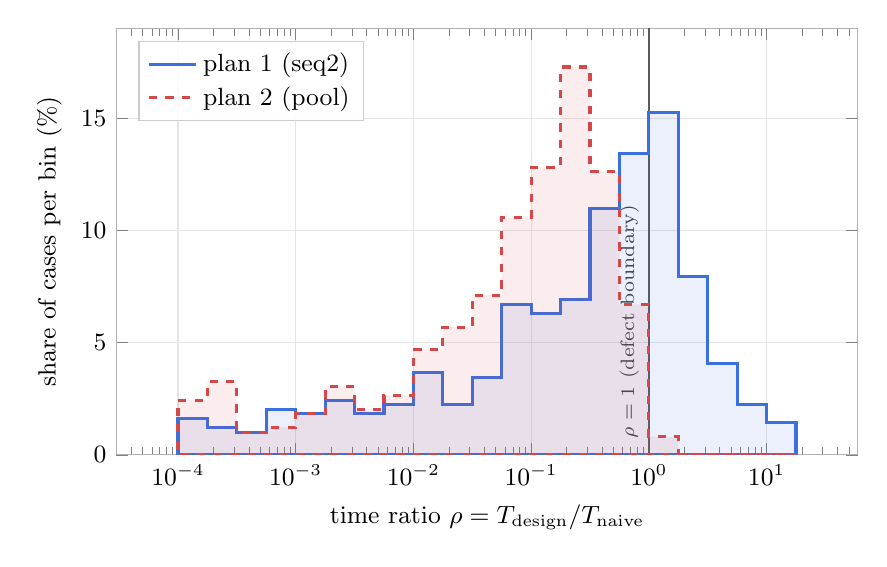
\begin{tikzpicture}
\begin{axis}[
  width=11cm, height=7cm,
  xmode=log,
  xlabel={time ratio $\rho = T_{\mathrm{design}} / T_{\mathrm{naive}}$},
  ylabel={share of cases per bin (\%)},
  ymin=0,
  grid=major, grid style={gray!20},
  axis line style={gray!60},
  tick label style={font=\small},
  label style={font=\small},
  legend style={at={(0.03,0.97)}, anchor=north west, font=\small,
                 draw=gray!40, fill=white, fill opacity=0.9, text opacity=1},
  legend cell align=left,
]
\draw[black!65, line width=0.9pt] (axis cs:1,0) -- (axis cs:1,\pgfkeysvalueof{/pgfplots/ymax});
\node[gray!50!black, font=\scriptsize, anchor=south west, rotate=90]
  at (axis cs:1,0.3) {$\rho=1$ (defect boundary)};
\addplot[seqblue, solid, line width=1.1pt, const plot,
  fill=seqblue, fill opacity=0.10, draw opacity=1] coordinates {
(0.0001,1.626)(0.000177828,1.220)(0.000316228,1.016)(0.000562341,2.033)(0.001,1.829)
(0.00177828,2.439)(0.00316228,1.829)(0.00562341,2.236)(0.01,3.659)(0.0177828,2.236)
(0.0316228,3.455)(0.0562341,6.707)(0.1,6.301)(0.177828,6.911)(0.316228,10.976)
(0.562341,13.415)(1,15.244)(1.77828,7.927)(3.16228,4.065)(5.62341,2.236)
(10,1.423)(17.7828,1.423)} \closedcycle;
\addlegendentry{plan 1 (seq2)}
\addplot[poolred, dashed, line width=1.1pt, const plot,
  fill=poolred, fill opacity=0.10, draw opacity=1] coordinates {
(0.0001,2.439)(0.000177828,3.252)(0.000316228,1.016)(0.000562341,1.220)(0.001,1.829)
(0.00177828,3.049)(0.00316228,2.033)(0.00562341,2.642)(0.01,4.675)(0.0177828,5.691)
(0.0316228,7.114)(0.0562341,10.569)(0.1,12.805)(0.177828,17.276)(0.316228,12.602)
(0.562341,6.707)(1,0.813)(1.77828,0.000)(3.16228,0.000)(5.62341,0.000)
(10,0.000)(17.7828,0.000)} \closedcycle;
\addlegendentry{plan 2 (pool)}
\end{axis}
\end{tikzpicture}
\end{document}
